\chapter{Marco tecnológico}\label{chap:tecnologia}

\section{Criterios de selección}

La selección tecnológica se guía por reproducibilidad, mantenibilidad, trazabilidad, capacidad de ejecución en un único equipo y disponibilidad de herramientas abiertas o de libre utilización. El objetivo no es acumular tecnologías, sino asignar una responsabilidad concreta a cada componente. La arquitectura final separa el movimiento y control operacional del dato, la transformación analítica, el aprendizaje automático y la visualización.

La solución se ejecuta sobre Windows con Docker Desktop, preferiblemente mediante integración WSL2. Los procesos de aplicación se encapsulan en contenedores Linux, reduciendo la dependencia del sistema anfitrión y permitiendo que el mismo repositorio pueda trasladarse posteriormente a un servidor Linux con cambios mínimos.

\section{Docker y Docker Compose}

Docker proporciona el mecanismo de aislamiento utilizado para empaquetar dependencias y procesos. Cada servicio se define mediante una imagen y un conjunto explícito de variables, volúmenes, redes y comprobaciones de salud. Docker Compose permite describir y ejecutar aplicaciones formadas por varios contenedores desde una especificación declarativa~\cite{docker_compose}.

En este trabajo, Compose reproduce la relación entre Apache NiFi, PostgreSQL, dbt, el entorno Python de machine learning, Redis y Superset. La plataforma debe poder arrancarse desde la raíz del repositorio mediante:

\begin{lstlisting}[language=bash,caption={Arranque general del entorno contenerizado.}]
docker compose up -d
\end{lstlisting}

Los directorios Bronze, los repositorios internos de NiFi que requieran persistencia, los modelos entrenados y la base de datos sobreviven a la recreación de los contenedores mediante volúmenes o montajes explícitos. Las credenciales de desarrollo se externalizan en variables de entorno o mecanismos equivalentes y nunca se incorporan al repositorio público.

\section{Apache NiFi}

Apache NiFi constituye la capa principal de ingesta y automatización del flujo de datos. Se trata de un sistema basado en programación por flujos que permite construir grafos dirigidos de enrutamiento, transformación e intermediación mediante una interfaz web~\cite{nifi_components}. En la arquitectura del TFM se utiliza para descubrir activos, realizar peticiones HTTP, controlar el estado de ficheros, enrutar errores, escribir Bronze, coordinar accesos a PostgreSQL y desencadenar las fases posteriores.

La elección de NiFi responde especialmente a cuatro capacidades. En primer lugar, cada procesador puede configurarse con planificación temporal o basada en expresiones CRON, evitando mantener un scheduler separado para la ingesta~\cite{nifi_user_guide}. En segundo lugar, los \textit{Process Groups} permiten encapsular subflujos y expresar la arquitectura de forma modular. En tercer lugar, los \textit{Parameter Contexts} desacoplan configuración de la lógica del flujo y permiten distinguir parámetros sensibles y no sensibles. Finalmente, el subsistema de \textit{Data Provenance} registra eventos asociados al recorrido de los FlowFiles, facilitando diagnóstico, linaje y auditoría~\cite{nifi_user_guide}.

La implementación organiza el canvas mediante grupos de procesos dedicados a control, descubrimiento, descarga, validación, fuentes externas, ejecución de dbt, disparo del proceso de ML y tratamiento de errores. Esta estructura se desarrolla con el propósito de que el flujo pueda entenderse tanto a nivel operativo como en la defensa académica del proyecto.

\section{NiFi y PostgreSQL}

NiFi se conecta a PostgreSQL mediante servicios JDBC administrados como \textit{Controller Services}. La documentación oficial proporciona servicios de \textit{connection pooling} y procesadores capaces de ejecutar SQL o escribir registros en una base relacional~\cite{nifi_dbcp,nifi_putdbrecord}. En el TFM, PostgreSQL es la fuente de verdad para el estado persistente del pipeline: ejecuciones, activos descubiertos, estados de ingesta y resultados de calidad.

Esta decisión evita depender exclusivamente del estado interno de NiFi. La procedencia de NiFi aporta trazabilidad del recorrido de cada FlowFile, mientras que las tablas del esquema \texttt{control} ofrecen una vista relacional, estable y consultable de las ejecuciones. Ambos mecanismos son complementarios.

\section{Apache Parquet}

Parquet es un formato columnar diseñado para almacenamiento y recuperación eficientes~\cite{parquet_docs}. Su utilización en Bronze está condicionada por la propia fuente, ya que la TLC distribuye los registros mensuales en este formato~\cite{nyctlc_tripdata}. Mantener el fichero original evita una conversión temprana innecesaria y permite explotar lectura selectiva de columnas y compresión.

La estructura de carpetas particiona lógicamente por dominio, servicio, año y mes. NiFi escribe cada activo únicamente cuando la transferencia y las validaciones mínimas han finalizado correctamente. La presencia física del fichero se acompaña siempre de metadatos en PostgreSQL\@.

\section{PostgreSQL}

PostgreSQL actúa como almacén relacional central para las capas Silver y Gold, además de contener los esquemas de control, auditoría y cuarentena. Se elige por su madurez, soporte SQL, ecosistema, capacidad de indexación y facilidad de integración con Docker~\cite{postgres_docs}.

La solución utiliza varios esquemas lógicos, previsiblemente \texttt{control}, \texttt{silver}, \texttt{gold} y \texttt{quarantine}. PostgreSQL no se utiliza como almacenamiento primario de Bronze, porque duplicar todos los ficheros originales incrementaría de forma sustancial el espacio utilizado sin aportar valor equivalente.

\section{dbt}

\textit{data build tool} (dbt) se utiliza para transformar datos accesibles al motor relacional.\ dbt permite definir modelos SQL con dependencias explícitas, ejecutar pruebas y generar documentación del grafo de transformación~\cite{dbt_docs}. De este modo, la lógica Silver y Gold permanece declarativa, versionada y separada del flujo operacional de NiFi.

La organización distingue modelos de \textit{staging}, Silver, Gold y \textit{marts}. NiFi puede desencadenar una ejecución de dbt cuando el conjunto de entrada requerido está disponible, pero no absorbe la lógica analítica que corresponde a los modelos SQL\@. Esta separación evita construir transformaciones complejas mediante un canvas visual cuando pueden expresarse con mayor claridad en SQL versionado.

\section{Python}

Python se mantiene como lenguaje principal de la capa de machine learning y para utilidades que requieran lógica de propósito general. Se utiliza para preparación de features no resueltas en SQL, entrenamiento, validación temporal, cálculo de métricas, persistencia de artefactos e inferencia.

Las primeras pruebas de ingesta y orquestación se realizaron con scripts Python. Esta implementación se conserva en el repositorio bajo una carpeta independiente, \texttt{Ingesta Python/}, como evidencia de la evolución arquitectónica y como referencia funcional. Tras validar la viabilidad del pipeline, se optó por Apache NiFi para la ingesta principal, al ofrecer una solución más reproducible y mantenible para programar, enrutar, reintentar y supervisar los flujos. Python se mantiene en la arquitectura para la preparación de variables, el entrenamiento y la inferencia de los modelos.

\section{scikit-learn}

scikit-learn proporciona una interfaz consistente para preprocesamiento, evaluación y modelos clásicos de aprendizaje automático~\cite{pedregosa2011}. En este trabajo se utiliza para la regresión de Poisson, Random Forest, métricas y utilidades de pipeline.

La selección de \texttt{PoissonRegressor} responde a la naturaleza de conteo del objetivo~\cite{sklearn_poisson}; \texttt{RandomForestRegressor} representa un ensemble de bagging capaz de modelar relaciones no lineales~\cite{sklearn_rf}.

\section{LightGBM}

LightGBM es una implementación de gradient boosting basada en árboles optimizada para datos tabulares y grandes volúmenes~\cite{ke2017,lightgbm_docs}. Su API compatible con scikit-learn facilita incorporarlo al mismo marco de entrenamiento y evaluación.

La elección de LightGBM no presupone que sea el modelo ganador. Los resultados experimentales deberán justificar si su complejidad adicional se traduce en una mejora suficiente respecto a Random Forest, Poisson y el baseline estacional.

\section{Apache Superset}

Apache Superset es una plataforma de exploración y visualización de datos que puede conectarse a múltiples bases de datos y construir dashboards interactivos~\cite{superset_docs}. En este proyecto consume exclusivamente modelos Gold o vistas específicamente preparadas para BI\@. Se evita que los gráficos contengan lógica de transformación sustantiva que no exista también en el almacén de datos.

Esta decisión mejora la trazabilidad: cada KPI debe tener una definición reproducible en SQL/dbt y Superset se utiliza para presentar, filtrar y combinar los resultados.

\section{Redis}

Redis se incorpora como servicio auxiliar de Superset cuando la configuración seleccionada requiere caché o componentes asíncronos. No forma parte del modelo analítico ni contiene la fuente de verdad del proyecto.

\section{Git, GitHub y versionado de flujos}

Git registra la evolución del código y permite asociar decisiones y resultados a revisiones concretas~\cite{git_docs}. El repositorio público se utiliza además como mecanismo de entrega reproducible. El historial debe excluir secretos, ficheros de datos masivos y volúmenes de ejecución.

El versionado del flujo NiFi se diseña utilizando las capacidades de \textit{Flow Registry Client} basadas en Git introducidas en NiFi 2. La propia comunidad de Apache NiFi anunció en 2026 la deprecación de NiFi Registry y recomienda migrar hacia clientes integrados con GitHub, GitLab, Bitbucket o Azure DevOps~\cite{nifi_registry}. En este proyecto se prioriza la integración con GitHub para evitar desplegar un servicio Registry adicional y mantener el flujo junto al resto de artefactos del TFM\@.

Los valores sensibles utilizados por los clientes de registro no se almacenan en Git. La configuración versionada debe conservar la estructura del flujo y los parámetros no secretos, mientras que tokens y credenciales permanecen externalizados.

\section{Relación entre componentes}

La \cref{fig:tech-flow} resume las responsabilidades. NiFi recibe y enruta los datos de las fuentes, preserva Bronze y registra el estado operacional.\ dbt transforma las capas Silver y Gold sobre PostgreSQL\@. Python consume features Gold para entrenar y ejecutar modelos. Superset consulta marts y predicciones persistidas.

\begin{figure}[H]
\centering
\IfFileExists{00.Figures/02.Capitulos/03/tech_flow.pdf}{%
  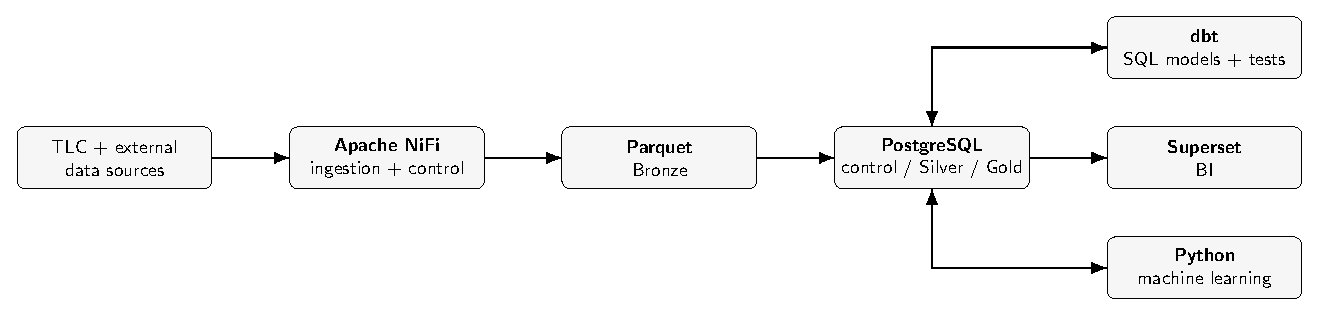
\includegraphics[width=0.96\textwidth]{00.Figures/02.Capitulos/03/tech_flow.pdf}%
}{%
  \missingfigurebox{tech\_flow.pdf}%
}
\caption{Relación funcional entre las principales tecnologías del proyecto con Apache NiFi como capa de ingesta y automatización.}%
\label{fig:tech-flow}%
\end{figure}

\section{Tecnologías deliberadamente no incorporadas}

No se introduce Airflow, Prefect o Dagster en la arquitectura principal. NiFi cubre la planificación y coordinación del flujo de ingesta, mientras que dbt mantiene el DAG de transformaciones SQL y Python se ocupa del ciclo de machine learning. Añadir un segundo orquestador incrementaría la superficie operativa sin una necesidad demostrada para el alcance local del proyecto.

Great Expectations fue considerado como herramienta adicional de contratos de calidad. En la versión NiFi se prioriza una distribución más simple de responsabilidades: validaciones físicas y de ruta en NiFi, reglas semánticas y tests relacionales en dbt, y validaciones específicas de ML en Python. Si durante la implementación se detecta una necesidad no cubierta, GX puede incorporarse de forma selectiva, pero no se considera requisito estructural.
